%!TEX root=../main.tex
\chapter{Network motifs}\label{sec:motifs}

Graphs representing networks, including biological networks and social networks, contain wide variety of subgraphs. One important local property of networks are so-called \emph{network motifs}, which are defined as recurrent and statistically significant sub-graphs or patterns.

Network motifs are sub-graphs that repeat themselves in a specific network or even among various networks. Each of these sub-graphs, defined by a particular pattern of interactions between vertices, may reflect a framework in which particular functions are achieved efficiently. Indeed, motifs are of notable importance largely because they may reflect functional properties.

Let's consider how motifs are used in social networks:
   \begin{itemize}
       \item To understand what is happening in a graph and build better algorithms;
       \item Classification: to find structural differences among graphs induced by different relations and measured counting the frequency of various motifs;
       \item Clustering: one can analyze the structure of a graph based on the cuts induced by the motifs instead of those induced by the edges (this approach turns out to be more accurate);
       \item Coordinate system: each subgraph (defined by some group or event on a social network, for example) becomes a point in the space based on the number of motifs.
   \end{itemize}

Let's start by the simplest network motifs, the triangles.


\section{Triangles}\label{sec:triangles}

The triangle is, unsurprisingly, defined as a triple of nodes for which each of the three pairs of node is connected. 
We would like to compute the \emph{global clustering coefficient}:
\begin{equation}\label{eq:clustering-coefficient}
    c(G) = \frac{3 \cdot \left(\text{\# triangles in G}\right)}{\left(\text{\# connected triples in G}\right)} = \frac{3 \mathcal{T}}{w(G)}.
\end{equation}
%
Let's compute this on an example.
%
\begin{figure}[h!]
	\centering
	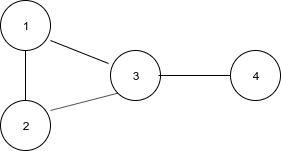
\includegraphics[width=.4\textwidth]{graph-triangle-example.png}
	\caption{Graph example}\label{fig:graph-example-triangles}
\end{figure}

In the graph shown in \cref{fig:graph-example-triangles} there are $5$ connected triples and $1$ triangle, so the global clustering coefficient would be $3/5$.
%
\begin{figure}[h!]
	\centering
	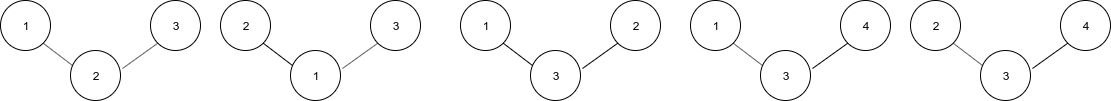
\includegraphics[width=\textwidth]{conn-triples.png}
\end{figure}

\obs The \emph{g.c.c.} for a clique is $1$, because every connected triple is also a triangle; while for a star it is $0$ because there are no triangles.

To compute the denominator for the \emph{g.c.c.}, that is $w(g)$, what we can do is sum all the pairs of nodes in the neighborhood of each node.
\[
	w(G) = \sum_{u \in V}\binom{deg(u)}{2}
\]
taking time $T = O(N)$.\\
This gives us a first algorithm to compute the \emph{g.c.c.}:
%
\begin{lstlisting}[caption={Algorithm 1}, label={lst:triangles-alg1}]
Algorithm_1:
    $\tau \gets 0$   // the number of triangles
    for $u \in V$:
        for $\{ v, w \} \in \binom{N_u}{2}$:   // where $N_u$ is the set of the neighbors of $u$
            if $\{ v, w \} \in E$:
                $\tau$ += 1
    return $\frac{\tau}{3}$
\end{lstlisting}
%
\begin{claim}\label{cl:triangles-1}
	Algorithm is in $O(n^3)$.
\end{claim}
\begin{proof}
    First, assume that we have both the adjacency matrix that represents the graph and the degree of each node.\\
    The complexity of the algorithm is given by $w(G)$, since we add at most 1 at each step, for each pair of nodes in $\binom{N_u}{2}$, thus,
	if the graph is dense -- that is the degree for each node $u$ is close to $n^2$ -- we have that:
	\[
		\sum_{u \in V}\binom{deg(u)}{2} = \sum_{u \in V}\Omega(n^2) = \Omega(n^3),
	\]
	while, if the \textit{max-degree} is constant, we have that:
	\[
		\sum_{u \in V}\binom{deg(u)}{2} = \sum_{u \in V} O(1) = O(n).
	\]
\end{proof}

Therefore, we would like to find other algorithms, or methods, to compute \textit{g.c.c.} faster, even for dense graphs.


\subsection{Adjacency Matrix method}\label{sec:triangles-adjacency}

One algorithm to compute the number of triangles is based on the adjacency matrix multiplication.
The adjacency matrix for the graph seen in \cref{fig:graph-example-triangles} is the following
\[
	A = \begin{pmatrix}
		0 & 1 & 1 & 0 \\
		1 & 0 & 1 & 0 \\
		1 & 1 & 0 & 1 \\
		0 & 0 & 1 & 0 \\
	\end{pmatrix}
\]
Let's compute the square of it.
\[
	A^2 = 	\begin{pmatrix}
		2 & 1 & 1 & 1 \\
		1 & 2 & 1 & 1 \\
		1 & 1 & 3 & 0 \\
		1 & 1 & 0 & 1 \\
	\end{pmatrix}
\]
Now, what does the $ij$ cell contain? By definition of matrix multiplication we have that
\[
	(A^2)_{uv} = \sum_{w \in G}A_{uw} \cdot A_{wv}
\]
where $A_{uw} = 1$ iff $(u,w) \in E$ and $A_{wv} = 1$ iff $(w,v) \in E$. In other words, we are counting the number of paths of length $2$ that go from $u$ to $w$.\\
In cell $A_{uu}$ there is the number of paths of length $2$ that go from $u$ to itself, that is equal to its degree because we can go from $u$ to any of its neighbours in $1$ step and then use the same edge to go back to $u$.\\
For $A^3$ we have that
\[
    (A^3)_{uv} = \left( A \cdot A^2 \right)_{uv} = \sum_{w \in G} A_{uw} \cdot (A^2)_{wv},
\]
thus, intuitively, $(A^3)_{uv}$ contains the number of paths of length $3$ that go from $u$ to $v$, and in general the same reasoning applies to any $A^k$ for paths of length $k$.

To find triangles we can compute $A^3$ and, for every node, get its diagonal entry in the matrix, effectively giving us the number of paths of length $3$ that go from that node to itself.

\begin{figure}[h!]
	\centering
	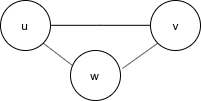
\includegraphics[width=.4\textwidth]{triangle.png}
	\caption{A triangle.}\label{fig:triangle-graph}
\end{figure}

Let's compute $(A^3)_{uu}$ in \cref{fig:triangle-graph}; there are two paths of length $3$ that go from $u$ to itself: $uvw, uwv$. So $(A^3)_{uu}$ would be $2$, but the node is in just one triangle.
That is true in general, so every triangle gives a contribute of $2$ to the diagonal entry of every node that forms it. Furthermore, this way we will count the same triangle $3$ times (1 for each vertex of the triangle).

\begin{defn}[Trace of a matrix]
    Let $m$ be a matrix, its trace is
    \begin{equation}\label{eq:trace}
        tr(M) = \sum_i M_{ii}.
    \end{equation}
\end{defn}

We thus have
\[
	\sum_{u \in G}{\left(A^3\right)_{uu}} = tr(A^3) = 6 \cdot \tau(G).
\]

\begin{thm}\label{thm:triangles-1}
    The number of triangles $\tau$ of a graph $G$ is given by
	$$\tau(G) = \frac{tr(A^3)}{6}.$$
\end{thm}

This gives us the following algorithm, that uses an algebraic approach based on the adjacency matrix it takes in input:
\begin{lstlisting}[caption={Algorithm 2}, label={lst:triangles-alg2}]
Algorithm_2(A):
    $AC \gets$ fast_mat_multiplication(A,3)
    return $tr(AC)/6$
\end{lstlisting}

\obs In general, to compute $A^i$, you need $\log_2(i)$ matrix multiplications.

\obs The execution time is given by the matrix multiplication, for which the best known algorithm takes time $O(n^{2.37})$, where $n$ is the number of nodes. Therefore, the complexity of [\ref{lst:triangles-alg2}] is independent from the number of edges, that is, the algorithm doesn't take into account the structure of the graph.\\
On the one hand this approach gives an improvement for dense graphs, for which we pass from $O(n^3)$ to $O(n^{2.37})$, while on the other hand we can get a worsening for sparse graphs, such as for the star, for which we pass from $O(n^2)$ to $O(n^{2.37})$.\\
Note that this is true because for a sparse matrix $A$, its square $A^2$ isn't sparse; consider the $A^2$ for a star, it is dense since there are a lot of possible two-paths.


\subsection{Structure-based method}\label{sec:triangles-structure}

Let's consider the star again, in algorithm [\ref{lst:triangles-alg1}] we loose a lot of time by making operations on the root node, that are useless, since we find the same ``potential triangles'' starting from the leaves.

\textit{Idea}: If we sort the nodes by their degree, and we follow this ordering when we look for triangles, we won't count the triangles more times, and we'll have less operations to do when we reach the nodes with higher degree (since we'll have already considered most of their neighbors).

\begin{ex}
    The ordering of the nodes of graph in figure [\ref{fig:graph-example-triangles}] is: \textit{4, 1, 2, 3}, since the degrees of the nodes are, respectively, \textit{1, 2, 2, 3}.
\end{ex}

This gives us the following algorithm:
\begin{lstlisting}[caption={Algorithm 3}, label={lst:triangles-alg3}]
Algorithm_3(G):
    $\tau \gets 0$
    $order(V) \gets$ sort $V$ so that $u < v \Longleftrightarrow  deg(u) \leq deg(v)$
    for each $u \in order(V)$:
        $N_u^+ \gets \{ v \in N_u \st v > u \}$
        for every $\{ v,w \} \in \binom{N_u^+}{2}$:
            if $\{ v,w \} \in E$:
                $\tau$ += 1
\end{lstlisting}

\begin{thm}\label{thm:triangles-2}
    \texttt{Algorithm\_3} [\ref{lst:triangles-alg3}] returns exactly $\tau(G)$.
\end{thm}
\begin{proof}
    Every triangle is counted exactly once by $w = \min \{ x \in triangle \}$, that is, the vertex with minimum degree in the triangle.
\end{proof}

\begin{thm}\label{thm:triangles-3}
    Let $\mathcal{E} = |E|$, \texttt{Algorithm\_3} [\ref{lst:triangles-alg3}] runs in $O(\mathcal{E}^{3/2})$.
\end{thm}

\ex Let's consider the star again, with Algorithm\_3 we need only $O(n^{1.5})$, instead of $O(n^2)$.

\obs Since we add at most 1 triangle at each step, there will be at most $O(\mathcal{E}^{3/2})$ triangles in the graph, furthermore \texttt{Algorithm\_3} [\ref{lst:triangles-alg3}] is able to return the whole list of triangles, along with their number.

\ex In a clique there are $\mathcal{E}^{3/2}$ triangles: $\mathcal{E} = \Theta(n^2),\ \tau(G) = \Theta(n^3) \Longrightarrow \tau(G) = \Theta(\mathcal{E}^{3/2})$. Then we cant do better than this in the worst case, but in general social graphs have less edges and so we can obtain better performances.

\begin{proof}[Proof of theorem \ref{thm:triangles-3}]
    We prove the theorem putting together some observations and lemmas.
    
    \begin{obs}\label{obs:triangles-1}
        First of all, consider that $\mathcal{E} = \frac12 \sum_{u \in G} deg(u)$, thus there are at most $2 \sqrt{\mathcal{E}}$ nodes with degree $\geq \sqrt{\mathcal{E}}$.
    \end{obs}
    
    Let $V_1 = \{ v \in V \st deg(v) \geq \sqrt{\mathcal{E}} \}$ and $V_2 = V - V_1 = \{ v \in V \st deg(v) < \sqrt{\mathcal{E}} \}$.\\
    By observation [\ref{obs:triangles-1}] we know that $|V_1| \leq 2 \sqrt{\mathcal{E}}$, then $E \geq \frac12 \sum_{u \in V_1} \sqrt{\mathcal{E}} = \frac12 |V_1| \sqrt{\mathcal{E}}$.
    
    \begin{obs}\label{obs:triangles-2}
        \begin{equation}\label{eq:triangles-t}
            T = \sum_{u \in V_2} \abs{\binom{N_u^+}{2}} \leq \sum_{u \in V} \abs{N_u^+}^2.
        \end{equation}
    \end{obs} % todo: is it V or V_1 ???

    \begin{lem}\label{lem:triangles-1}
        $\abs{N_u^+} \leq 2 \sqrt{\mathcal{E}}\ \forall\ u \in V_1$.
    \end{lem}
    \begin{proof}
        Refer to figure [\ref{fig:triangles-l1}].
        
        \begin{figure}[h!]
            \centering
            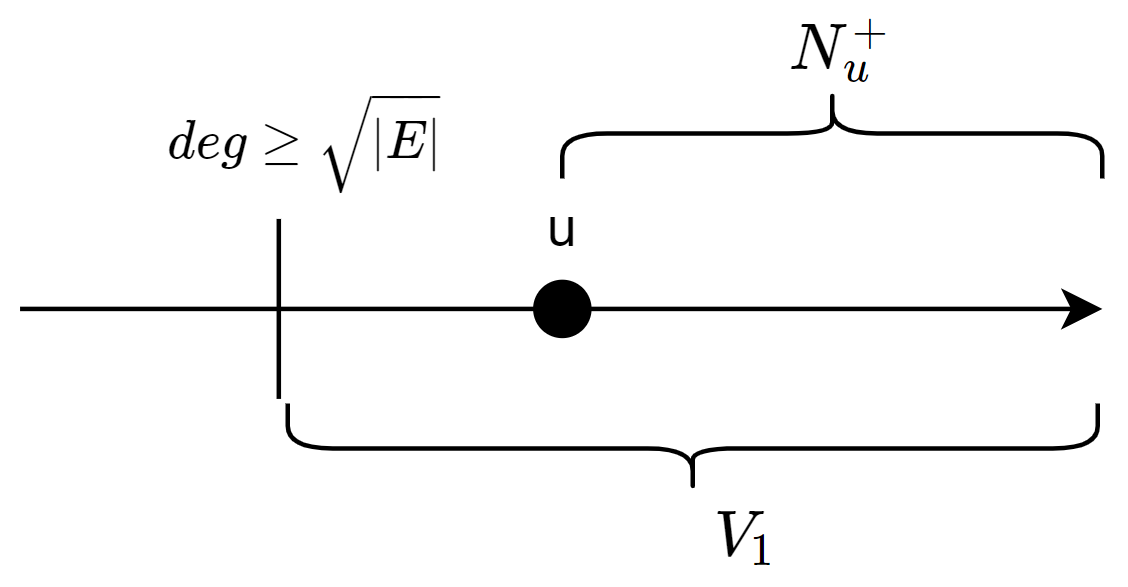
\includegraphics[width=.4\textwidth]{triangles_l1.png}
            \caption{A visual proof of lemma [\ref{lem:triangles-1}]}
            \label{fig:triangles-l1}
        \end{figure}
    \end{proof}

    Then we can define $T_{V_1}$ and give it an upper bound (this will allow us to prove an upper bound for $T$, together with $T_{V_2}$, that we'll define later):
    \begin{equation}\label{eq:triangles-tv1}
        T_{V_1} = \sum_{u \in V_1} \abs{\binom{N_u^+}{2}} \leq \sum_{u \in V_1} \abs{N_u^+}^2 \leq 8 \mathcal{E}^{3/2}.
    \end{equation}
    
    In order to give a similar bound to $T_{V_2}$, we partition the nodes in $V_2$ in buckets as follows, according with their degree:\\
    $V_2 = V_2^{(1)} \cup V_2^{(2)} \cup \ldots \cup V_2^{(i)} \cup \ldots \cup V_2^{(k)}$, where $V_2^{(1)} = \{ v \st v \in V \wedge \frac{\sqrt{\mathcal{E}}}{2} \leq deg(v) < \sqrt{\mathcal{E}} \}$, $V_2^{(2)} = \{ v \st v \in V \wedge \frac{\sqrt{\mathcal{E}}}{4} \leq deg(v) < \frac{\sqrt{\mathcal{E}}}{2} \}$, $V_2^{(i)} = \{ v \st v \in V \wedge \frac{\sqrt{\mathcal{E}}}{2^{i+1}} \leq deg(v) < \frac{\sqrt{\mathcal{E}}}{2^i} \}$, $V_2^{(k)} = \{ v \st v \in V \wedge 1 \leq deg(v) < 2 \}$.\\
    We know that $\abs{V_2^{(1)}} \leq 4 \sqrt{\mathcal{E}}$ by lemma [\ref{lem:triangles-1}], then we can compute $\abs{V_2^{(2)}} \leq \frac{2 \mathcal{E}}{\frac{\sqrt{\mathcal{E}}}{4}} = 8 \sqrt{\mathcal{E}}$, $\abs{V_2^{(i)}} \leq \frac{2 \mathcal{E}}{\frac{\sqrt{\mathcal{E}}}{2^{i+1}}} = 2^{i+1} \sqrt{\mathcal{E}}$.
    
    We can underline our last result in the following lemma:
    \begin{lem}\label{lem:triangles-2}
        \begin{equation}
            \abs{V_2^{(i)}} \leq 2^{i+1} \sqrt{\mathcal{E}}.
        \end{equation}
    \end{lem}

    \begin{lem}\label{lem:triangles-3}
        \begin{equation}\label{eq:triangles-tv2}
            T_{V_2} = \sum_{u \in V_2} \abs{\binom{N_u^+}{2}} \leq \sum_{u \in V_2} \abs{N_u^+}^2 \leq \sum_{u \in V_2} deg(u)^2.
        \end{equation}
    \end{lem}

    \begin{lem}\label{lem:triangles-4}
        For $u \in V_2^{(i)}$, \texttt{algorithm-3} [\ref{lst:triangles-alg3}] does at most $\mathcal{E} 2^{-2i}$ steps.
    \end{lem}

    Thus, we can conclude the proof of theorem by giving an upper bound for $T_{V_2}$, that -- together with the bound for $T_{V_1}$ shown in [\ref{eq:triangles-tv1}] -- will give us a bound for $T$ [\ref{eq:triangles-t}]:
    \begin{flalign*}
        T_{V_2} &= T_{V_2^{(1)}} + T_{V_2^{(2)}} + \ldots + T_{V_2^{(i)}} + \ldots + T_{V_2^{(k)}}&\\
        &= \sum_{i=1}^{\log_2 \sqrt{\mathcal{E}}} \left( \abs{V_2^{(i)}} \cdot \left(\text{ work for } u \in V_2^{(i)} \right) \right)&\\
        &= \sum_{i=1}^{\log_2 \sqrt{\mathcal{E}}} \left( 2^{i+2} \sqrt{\mathcal{E}} \cdot \mathcal{E}2^{-2i} \right)&\\
        &\leq \mathcal{E} \sqrt{\mathcal{E}} \cdot \sum_{i=1}^{\log_2 \sqrt{\mathcal{E}}} 2^{-2i} \leq 4 \mathcal{E}^{3/2}.&
    \end{flalign*}
\end{proof}


\section{Motifs with more than three nodes}\label{sec:big-motifs}

If we want to count the number of motifs with more than three nodes, it becomes increasingly difficult as the number of nodes we consider increases (for example, the problem of counting the number of cliques in a graph is NP-complete). For this reason, generally we look for an approximation of the optimal solution.

\begin{defn}
    Given a motif $H$ on $k$ nodes, let
    \begin{equation}\label{eq:motif}
        c_H = \abs{\{U \subseteq V : G[U] \simeq H\}}
    \end{equation}
    be the number of occurrences of the motif we are looking for in the graph.\\
    Note that $G[U] \simeq H$ means ``the subgraph on $G$ induced by $U$ is isomorphic to $H$''. 
\end{defn}

Thus, our goal is to obtain an estimate $\hat{c}_H$ of $c_H$ such that $c_H - t \leq \hat{c}_H \leq c_H + t$ with probability $1-p$.\\
Note that this resembles what we've done with Randomized Pivot algorithm for Correlation clustering (see [\ref{thm:clust-rp-approx}]).

Since it would take an exponential amount of time to pick each subgraph of $k$ nodes and check if it is isomorphic to $H$, we'll use sampling (see [\ref{def:sampling}]).

\begin{lstlisting}[caption={Algorithm 1}, label={lst:motifs-alg1}]
Algorithm_1(G, H):
    $U \gets \left\lbrace k \text{ nodes sampled } \uar \text{ from } \binom{V}{k} \right\rbrace$;
    $F \gets G[U]$;
    return $Y_H = \mathbbm{1}[F \simeq H]$;
\end{lstlisting}
Note that, to evaluate the characteristic function $\mathbbm{1}$, that returns 1 if the argument is true and 0 otherwise, it takes only constant time, since we are considering only $k$ nodes, and so we'll need to verify at most $k!$ permutations of the nodes in $U$.

Now let's analyze the expected value of the output of the algorithm:
\begin{equation}\label{eq:eyh-1}
    E[Y_H] = \frac{\sum_{F \subseteq G, F \simeq H} 1}{\binom{|V|}{k}} = \frac{c_H}{\binom{n}{k}} = \sum_{F \subseteq G, F \simeq H} \frac{1}{\binom{n}{k}}
\end{equation}
That is, the number of subgraphs of $G$ that are isomorphic to $H$ over the number of all the subrapgs of $G$ of size $k$.

\begin{obs}
    The expected value of the solution returned by Algorithm 1 [\ref{lst:motifs-alg1}] is linear with respect to $c_H$, but we would like to obtain an unbiased estimator of $c_H$, i.e., a random variable $X_H$ such that $E[X_H] = c_H$. We can define it as follows:
    \begin{equation}\label{eq:exh-1}
        X_H = \binom{n}{k} \cdot Y_H.
    \end{equation}
    In this way, the expected value is what we want, but the variance is very high: a single sample gives us 0 or $\binom{n}{k}$, nothing very useful, and we can't pick $\binom{n}{k}$ samples.
\end{obs}

\begin{obs}
    Since $H$ is connected, if we apply Algorithm 1 [\ref{lst:motifs-alg1}] on a sparse graph, we'll perform many useless samplings (we'll pick unconnected subgraphs with high probability). For example, the probability of peaking a $k$-motif on a star is $k/n$. Thus, we can slightly modify the algorithm as follows:
    \begin{lstlisting}[caption={Algorithm 1b}, label={lst:motifs-alg1b}]
Algorithm_1b(G, H):
    $U \gets \left\lbrace k \text{ nodes sampled } \uar \text{ from } \binom{V}{k} \right\rbrace$;
    $F \gets G[U]$;
    if $F$ is not connected:
        return "FAIL";
    else:
        return $Y_H = \mathbbm{1}[F \simeq H]$;
    \end{lstlisting}
    But this doesn't produce a big improvement, so how can we pick $k$ nodes in such a way that they are connected, and so they have the possibility to form the motif we are looking for? A possibility is to pick a random node, then choose one of its neighbors, then choose a neighbor of the selected neighbor, and so on. We'll describe an algorithm to do this for a special case: the 4-motif.
\end{obs}


\subsection{4-motifs}\label{sec:4-motifs}

Let's consider different examples of motifs with 4 nodes, shown in figure [\ref{fig:4-motifs}].

\begin{figure}[h!]
    \centering
    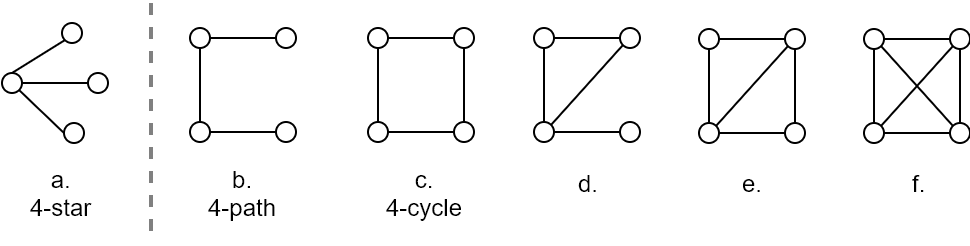
\includegraphics[width=0.9\textwidth]{4-motifs}
    \caption{Examples of 4-motifs}
    \label{fig:4-motifs}
\end{figure}

\obs The star (a.) can be considered a special case, since it doesn't contain any 4-path.

\obs Considering 4-motifs from b. to f., if we use the procedure mentioned at the end of the previous section (\textit{sample a random node, choose one of its neighbors, choose a neighbor of the selected neighbor, and so on}), these motifs have different probabilities to be found, since they have different number of 4-paths (increasing from b. to f.).

Let's describe an algorithm for finding the 4-paths (b.) in a graph:
\begin{lstlisting}[caption={Algorithm 2 (Path sample)}, label={lst:motifs-alg2}]
Algorithm_2(G):
    choose $u_1\ \uar$ from $V$
    for $i = 2,3,4$:
        choose $u_i\ \uar$ from $N_{u_{i-1}}$   // $N_x$ is the set of the neighbors of $x$
    return $Y_H = \mathbbm{1}[F \simeq H]$;
\end{lstlisting}

Let's study the expected value of the result of \texttt{Path sample}.\\
Let $a,b,c,d$ be nodes in $G$ that form a 4-path, note that the algorithm can pick the path $a \to b \to c \to d$ or the path $d \to c \to b \to a$.
\begin{flalign}
    E[Y_H] &= \sum_{F \subseteq G, F \simeq H} \Pr{\text{\texttt{Path sample} hits }F} =&\\
    &= \sum_{F \subseteq G, F \simeq H} \left( \frac1n \cdot \frac{1}{deg(a)} \cdot \frac{1}{deg(b)} \cdot \frac{1}{deg(c)} + \frac1n \cdot \frac{1}{deg(d)} \cdot \frac{1}{deg(c)} \cdot \frac{1}{deg(b)} \right)&\\
    &= \sum_{F \subseteq G, F \simeq H} \left( \frac{1}{n \cdot \deg(b) \cdot \deg(c)} \left( \frac{1}{deg(a)} + \frac{1}{deg(d)} \right) \right)&\\
    &= \sum_{F \subseteq G, F \simeq H} \sigma_F&\label{eq:eyh-2}
\end{flalign}

\obs While the probability of hitting any node in \texttt{Algorithm 1} [\ref{lst:motifs-alg1}] was uniform, and so we had a sum of the same value for each $F$, the probability of sampling a node in \texttt{Path sample} [\ref{lst:motifs-alg2}] depends on the degrees of the previous picked nodes, except for the first chosen node, picked $\uar$. Thus, the probability of finding a certain path depends on the degrees of the nodes that compose it, so an isolated path, where each node has degree 1 or 2, has higher probability of being chosen than any other path.

To obtain an expected value of $c_H$, we need to remove this unbalancing, so we apply a compensation factor to $Y_H$, similarly to what we did in [\ref{eq:exh-1}]:
\begin{equation}\label{eq:exh-2}
    X_H = \frac{1}{\sigma_F} \cdot Y_H.
\end{equation}

Let $Y_F := \mathbbm{1}[\text{\texttt{Path sample} hits }F]$ (bernoullian random variable) and $X_F := Y_F \cdot \frac{1}{\sigma_F}$, then
\begin{flalign*}
    \Var(X_F) &= \Var(Y_F \cdot \frac{1}{\sigma_F}) =\\
    &= \frac{1}{\left(\sigma_F\right)^2} \cdot \Var(Y_F)&\\
    &= \frac{1}{\left(\sigma_F\right)^2} \cdot \left( \sigma_F \cdot (1 - \sigma_F) \right)&\\
    &= \frac{1}{\left(\sigma_F\right)^2} \cdot \sigma_F -1&\\
    &\leq \frac{1}{\sigma_F} = O\left(n \cdot \Delta^3\right)&
\end{flalign*}
where $\Delta$ is the maximum degree of the graph. Thus, if the graph is sparse (the degree is constant), $\Var(X_F) = O(n)$.

At this point, it's important to note that there is a problem in the algorithm [\ref{lst:motifs-alg2}]: when we choose a node $u_i$, a neighbor of $u_i$, $u_{i+1}$, and we look for a neighbor of $u_{i+1}$, we could pick $u_i$ again, thus picking a path with less than 4 nodes. But it isn't difficult to overcome this problem, for example by going back to the second step of the algorithm if $F$ does not contain 4 nodes.\\
Thus, \texttt{Path sample} is a \textbf{rejection sampling} algorithm, i.e., one pick new elements at random and increment a counter if they match some criterion, otherwise the elements are thrown away.

\obs A strength of the algorithm is that it actually produces the list of the motifs it founds, not only their number. This behavior is similar to that of \texttt{Algorithm 3} for triangles [\ref{lst:triangles-alg3}] but opposite to that of \texttt{Algorithm 2} for triangles [\ref{lst:triangles-alg2}].

\obs For other kind of motifs, one can use the same algorithm, but the probability $\sigma_F$ will change.
